\documentclass[../main.tex]{subfiles}

\begin{document}
    The function of this repository is pretty simple:
    \begin{itemize}
        \item {
            \code{main.tex}: organizes main document and inserts subfiles in the correct order in the correct sections

            Additional configuration is further broken out into the files:
            \begin{itemize}
                \item \code{packages.tex}: any packages you want to use
                \item \code{bigtex-macros.sty}: reusable user-defined macros
                \item \code{document-macros.tex}: document- or domain-specific macros
                \item \code{config.tex}: any document configuration \emph{that can be placed outside of \code{main.tex}}
            \end{itemize}
        }
        \item \code{chapters/*.tex}: anything you want to insert as a subfile in \code{main.tex}
        \item \code{figures/}: any figures you want to include in your chapters
    \end{itemize}

    \subsection{A Picture of a Frog}
    \begin{figure}[h!]
        \centering
        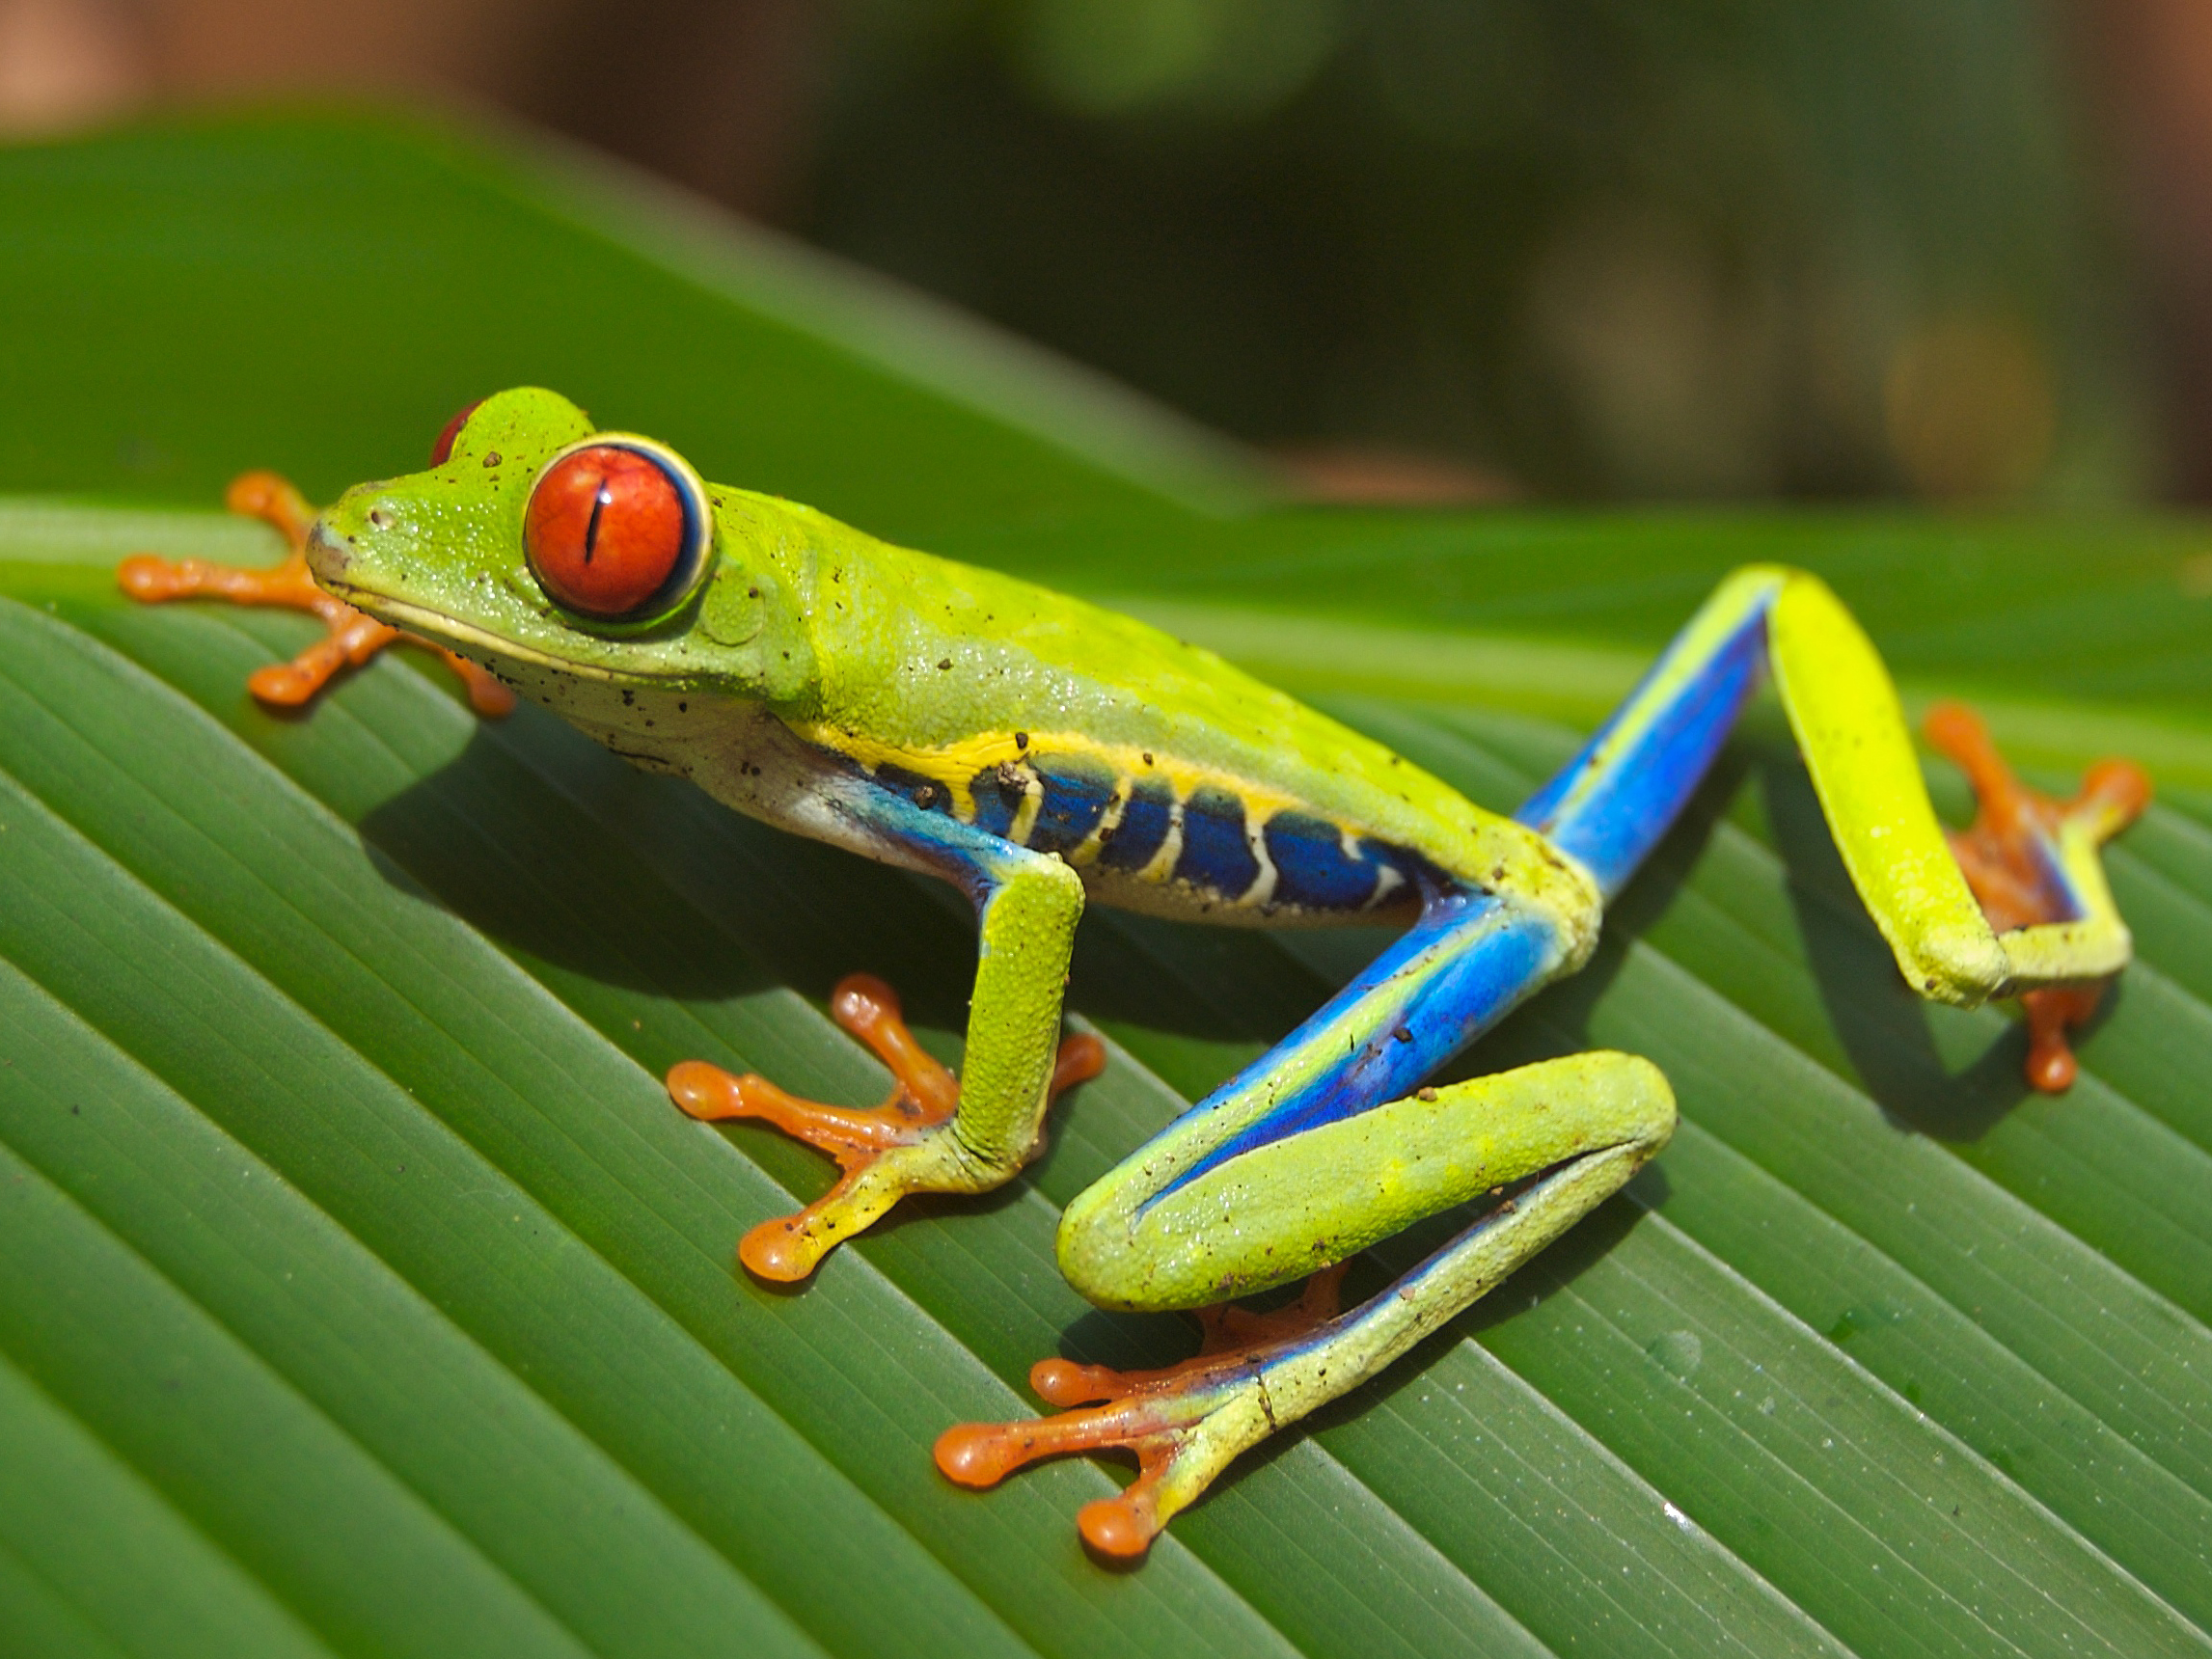
\includegraphics[width=0.6\textwidth]{../figures/methods/frog.jpg}
        \caption{An image of a frog.}
    \end{figure}

    \subsection{Lipsum Text, Section II}
    \lipsum[2]
\end{document}
